% Indicate the main file. Must go at the beginning of the file.
% !TEX root = ../main.tex

%----------------------------------------------------------------------------------------
% CHAPTER TEMPLATE
%----------------------------------------------------------------------------------------


\chapter{Methodology} % Main chapter title

\label{ChapterMethodology} % Change X to a consecutive number; for referencing this chapter elsewhere, use \ref{ChapterX}

%----------------------------------------------------------------------------------------
% SECTION 1
%----------------------------------------------------------------------------------------

\section{Materials and Dataset}

\subsection{Dataset Description}

The experiments we conducted in this thesis are all based on a large scale news article corpus derived from the CC-News dataset, as made available through the Hugging Face repository \cite{ccnews}. The dataset consists of news articles crawled from a wide range of online news sources and spans a time period from 2016 to 2021, making it very suitable for longitudinal analysies of media narratives and public perception.

The entirity of the dataset contains approximately 134 million rows of news articles, amounting to around 221 GB of compressed parquet files. Each entry in the dataset includes heading, publication year, source URL and a raw text field containing the article body. The articles cover a diverse set of topics, including politics, technology, finance, health, entertainment and more. The wide topical coverage and large scale of the dataset make it well-suited for analyzing trends and shifts in public discourse over time.

For the purpose of this thesis, a reduced cross-section of this dataset was used. Approximately 10\% of the original corpus was sampled, resulting in our working dataset of roughly 13 million articles. The reduction was necessary to ensure feasible processing times and resource requirements. Given the exploratory nature of this thesis, the reduced dataset still provides sufficient coverage and diversity to evaluate the proposed system and conduct meaningful analyses.

Each entry in the dataset inlcudes heading, publication year, source URL and a raw text field containing the article body.

\begin{table}[!htbp]
    \centering
    \caption{Example news article entry from the CC-News dataset (content truncated for readability).}
    \label{tab:dataset-example}
    \renewcommand{\arraystretch}{1.2}
    \begin{tabular}{|l|p{10cm}|}
        \hline
        \textbf{Field} & \textbf{Value}                                                                                                                                                                                \\
        \hline
        Title          & Samsung Names Scion Lee Jae-Yong to Board Of Directors                                                                                                                                        \\
        \hline
        Year           & 2016                                                                                                                                                                                          \\
        \hline
        Source Domain  & hamodia.com                                                                                                                                                                                   \\
        \hline
        Article ID     & 397547                                                                                                                                                                                        \\
        \hline
        Body (snippet) &
        Monday, September 12, 2016 at 2:09 pm.
        Lee Jae-yong (AP Photo/Ahn Young-joon, File).
        Samsung Electronics vice chairman Lee Jae-yong was nominated to join its board of directors. The announcement comes as the company grapples with a major smartphone recall affecting millions of devices\ldots \\
        \hline
    \end{tabular}
\end{table}

Table \ref{tab:dataset-example} shows an example entry from the CC-News dataset, illustrating the structure and content of a typical news article record. The body field has been truncated for readability.

\pagebreak

\subsection{Dataset Motivation}

Our main objective with this thesis was to explore how LLMs can be effectively combined with classical NLP methods to answer complex, temporally-aware analytical questions over large text corpora. A news corpus was selected as the underlying data source both due to its relevance for studying changes in media coverage and becuase news articles serve as a natural proxy for analyzing public discourse, media framing and shifts in perception over time.

Questions such as how the portrayal of a topic or the opinion on a public figure evolves across years, or how sentiment and narrative emphasis shift in response to major events are inherently temporal in nature. Therefore, large volumes of text spanning multiple time periods are required to capture these dynamics.

Prior to selecting this CC-Newes corpus, alternative datasets such as the CNN/DailyMail corpus \cite{cnndailymail} were considered. However, these datasets were ultimately deemed less suitable due to the lack of reliable temporal metadata beyond article content and headlines, which limited their suitability for time-based analysis. While the selected CC-News dataset provides temporal information primarily at the year level rather than at a fine-grained date resolution, it still enables meaningful year-over-year comparisons and trend analyses, which aligns with the goals of this thesis.

The suitability of news corpora for diachronic analysis has also been demonstrated in prior work. For example, Marjanen et al.~\cite{marjanen2020topic} apply topic modeling techniques to historical newspaper collections in order to study long-term discourse dynamics and shifts in dominant narratives over time. This supports our choice of a temporally structured news corpus as the empirical basis for a pipeline that combines classical topic-oriented analysis with LLM-based synthesis.

\subsection{Dataset Variants / Preprocessing}

The CC-News dataset has already undergone several preprocessing and quality assurance steps prior to its release. Non-English documents are removed and low quality content such as advertisements is filtered using heuristic methods. Additionally, the dataset is globally deduplicated and cross-deduplicated against external corpora such as OpenWebText2, resulting in the removal of approximately 0.3 million documents \cite{openwebtext2}.

Beyond the dataset's native preprocessing, no additional manual cleaning or annotation was applied in this thesis. Articles were filtered primarily by language, minimum text length, and year-based slicing to support temporal analysis. This design choice reflects our goal emphasis on scalable, automated exploration rather than curated or manually labeled datasets.

\subsection{Data Storage and Indexing Infrastructure}

To efficiently manage and query the large dataset, the corpus is stored using a multi-layer data management architecture. Primarily, a PostgreSQL is used to store the complete dataset as the authoritative source of truth for all articles. This choice enables flexible schema adjustment and supports future extensions of the dataset.

For efficient text retrieval, an OpenSearch index is constructed over selected textual fields. OpenSearch provides optimized inverted indexing based on the Lucene engine, enabling fast keyword-based retrieval over millions of documents. Inverted index–based retrieval systems commonly rely on probabilistic ranking functions such as BM25 \cite{manning2008ir,robertson2009bm25}, which score documents based on term frequency, inverse document frequency, and document length normalization:

\begin{equation}
    \text{BM25}(q, d) = \sum_{t \in q}
    IDF(t) \cdot
    \frac{f(t,d)\,(k_1 + 1)}
    {f(t,d) + k_1 \left(1 - b + b \cdot \frac{|d|}{\text{avgdl}}\right)}
\end{equation}

The BM25 ranking function scores documents based on how frequently and distinctively query terms occur in each document, while normalizing for document length to ensure fair comparison across heterogeneous text sources.

%----------------------------------------------------------------------------------------
% EVALUATION QUESTION SET AND EXPERIMENTAL DESIGN
%----------------------------------------------------------------------------------------

\section{Evaluation Question Set and Experimental Design}

\subsection{Rationale and Design Goals}

To evaluate the proposed CorpusAgent pipeline beyond anecdotal demonstrations, we define a structured set of evaluation questions that act as a task-oriented benchmark for the system. The goal of this question set is not to test factual question answering in isolation, but rather to assess whether a multi-stage pipeline can (i) retrieve relevant evidence from a large corpus, (ii) extract structured signals using classical NLP components, (iii) aggregate these signals across time, and (iv) synthesize an interpretable, verifiable narrative answer grounded in the retrieved material.

The questions were selected to cover diverse topical domains (politics, technology, finance, public health, climate discourse), different temporal dynamics (slow narrative shifts versus event-driven changes), and varying degrees of required tool composition. In addition, the set includes explicit negative and counterfactual controls to test robustness against spurious correlations and unsupported premises. This design reflects the dual objectives of demonstrating the analytical capabilities of the pipeline while also probing its reliability and interpretability properties.

Most of the questions are temporal based and therefore require evidence aggregation across multiple years. Studies have demonstrated the value of longitudinal sentiment analysis in news corpora for tracking how emotional tenor and polarity evolve over extended periods \cite{10.1371/journal.pone.0276367}.

\subsection{Question Categories}

The evaluation questions are grouped into four categories, each targeting a specific capability of the system:

\textbf{(A) Core longitudinal questions.}
These questions represent the primary target use case of the system: temporally-aware analysis of media narratives and tone over multi-year periods (2016--2021). They require evidence aggregation across time and typically involve one or more external signals for contextualization.

The question in this category:
\begin{itemize}
    \item A1 - Trump: media sentiment vs US market volatility \\ \textit{How did media sentiment towards Donald Trump evolve from the 2016 campaign through the end of his presidency (2016–2020), and how did it align with volatility spikes in VIX / S\&P 500 drawdowns around major events (election night, travel ban, trade-war escalations, impeachment, COVID crash)?}
    \item A2 - Facebook / Cambridge Analytica: shift to "techlash" + stock drawdowns \\ \textit{How did Facebook coverage shift from innovation/growth framing to privacy/regulation framing around the Cambridge Analytica scandal (2016–2019), and how did this correspond to FB stock drawdowns?}
    \item A3 - COVID-19: tone + topic evolution across phases \\ \textit{How did media tone and dominant themes around COVID-19 evolve from outbreak (late 2019/early 2020) to vaccine rollout (2021), and how did health vs economy vs civil-liberty frames compete over time?}
    \item A4 - Greta Thunberg / youth climate activism: framing across regions \\ \textit{How did media coverage of Greta Thunberg and youth climate activism evolve (2018–2021), and how did framing differ by region/outlet type (personalization vs policy vs skepticism/backlash)?}
    \item A5 - Crypto cycles: tone/themes vs BTC market phases \\ \textit{How did media tone and themes around Bitcoin/crypto change across the 2017 bull run, 2018 crash, and 2020–2021 bull market, and how did topic shifts align with BTC turning points?}
    \item A6 - Tesla/EV mainstreaming: hype vs safety vs market acceptance \\ \textit{How did media sentiment towards Tesla/EVs evolve (2016–2021), especially around Autopilot accidents, Model 3 production issues, and S\&P 500 inclusion, and how did this align with TSLA price moves?}
    \item A7 - US–China trade war \& Huawei/5G: competing frames \\ \textit{How did Western media coverage of Huawei and the US–China trade war evolve (2018–2021), and how did security vs economic vs tech-innovation frames compete across regions?}
    \item A8 - Brexit negotiations: coverage tone vs GBP volatility \\ \textit{How did media tone and key themes around Brexit evolve from the 2016 referendum through the UK's exit process (2016–2020), and how did sentiment/topic shifts align with GBP volatility around major milestones (Article 50, deal votes, extensions, withdrawal agreement)?}
\end{itemize}

\textbf{(B) Multi-hop / tool-composition questions.}
These questions are designed to test whether the agent can resolve an indirection step prior to corpus retrieval. Concretely, the system must first determine a canonical entity from an oblique description (e.g., "the company that owns Instagram"), identify an appropriate temporal anchor (e.g., a key event date or window), and only then execute the corpus pipeline. This category primarily evaluates planning and tool orchestration rather than raw retrieval.

The questions in this category:
\begin{itemize}
    \item B1 - Spouse indirection (Bill Gates → Melinda French Gates) + 2021 divorce \\ \textit{How did media coverage of the spouse of the Microsoft co-founder who runs a major philanthropic foundation change around the 2021 divorce announcement?}
    \item B2 - Parent company (Instagram → Facebook/Meta) around Cambridge Analytica \\ \textit{How did media sentiment towards the company that owns Instagram change before vs after the Cambridge Analytica scandal?}
    \item B3 - Role + other company (SpaceX founder → Tesla) + SEC settlement (2018) \\ \textit{How did media coverage of the electric-car company led by the founder of SpaceX change after the 2018 SEC settlement over tweets?}
    \item B4 - Movement figurehead ("How dare you" UN 2019 → Greta Thunberg) \\ \textit{How did global media coverage of the youth climate activist behind the "How dare you" UN speech change between 2018 and 2021?}
    \item B5 - Owner/brand mapping (WhatsApp → Meta) + encryption/data-sharing debate \\ \textit{How did media tone towards the company that owns WhatsApp change around the 2016–2017 encryption and data-sharing debates?}
    \item B6 - Product → parent company (TikTok → ByteDance) + US ban pressure \\ \textit{How did media tone towards the company that owns TikTok evolve around the 2020–2021 US ban / divestment pressure, and did the dominant framing shift between "national security" vs "tech/consumer product" vs "geopolitics"?}
\end{itemize}

\textbf{(C) Negative-control questions.}
Negative controls are intentionally constructed such that no meaningful relationship should be detectable. For these questions, correct behavior is not the construction of an elaborate narrative, but an explicit conclusion that no robust relationship is supported by the retrieved data, accompanied by brief diagnostic justification (e.g., weak and unstable correlations, low coverage volume, or inconsistent effects across time).

The questions in this category:
\begin{itemize}
    \item C1 - Bitcoin vs consumer staples sentiment (Colgate-Palmolive) \\ \textit{Did Bitcoin price movements (2016–2021) have any systematic impact on media sentiment towards Colgate-Palmolive?}
    \item C2 - Oscars vs US bank sentiment \\ \textit{Did the number of Oscars won in a year meaningfully affect media sentiment toward major US banks (JPM, BAC, etc.) from 2016–2021?}
    \item C3 - Zurich weather vs OPEC sentiment \\ \textit{Is there any meaningful relationship between daily weather in Zurich and media sentiment towards OPEC decisions (2016–2021)?}
    \item C4 - eSports results vs central bank policy coverage \\ \textit{Did major eSports tournament results (e.g., LoL Worlds winners) cause measurable shifts in sentiment about Fed/ECB policy (2016–2021)?}
\end{itemize}

\textbf{(D) Counterfactual / impossible-event controls.}
Finally, a small set of plausible-sounding questions is included where the premise is false (i.e., the referenced event did not occur). This category tests whether the system can detect unsupported assumptions and respond conservatively. In such cases, a correct answer must explicitly flag the premise as incorrect or not supported by evidence, rather than attempting to "fill in" a narrative by hallucination.

Concerns about model trustworthiness and explanation fidelity have been widely discussed in the machine learning literature, motivating the inclusion of negative and counterfactual questions to reduce overconfidence in model outputs \cite{ribeiro2016whyitrustyou}.

The questions in this category:
\begin{itemize}
    \item D1 - "Meta rebrand in 2018" (counterfactual) \\ \textit{How did media sentiment toward Facebook change after the company rebranded to "Meta" in 2018, and did coverage shift toward "metaverse" framing immediately afterward (2018–2019)?}
    \item D2 - "Amazon spun off AWS in 2019 IPO" (counterfactual) \\ \textit{How did media coverage of Amazon change after it spun off AWS via a separate IPO in 2019, particularly regarding antitrust and valuation framing (2018–2020)?}
\end{itemize}

With these four categories, we aim to comprehensively evaluate the capabilities of the proposed CorpusAgent pipeline across a range of realistic and challenging scenarios.

%----------------------------------------------------------------------------------------
% OVERVIEW OF THE PROPOSED SYSTEM
%----------------------------------------------------------------------------------------

\section{Overview of the Proposed System}

\begin{figure}[ht]
    \centering
    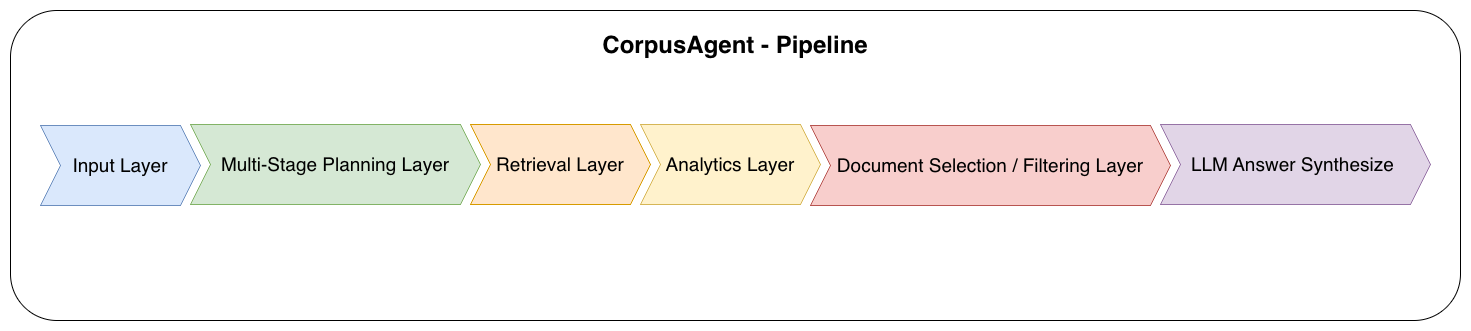
\includegraphics[width=1\textwidth]{Figures/Pipeline-Overview.png}
    \caption{Pipeline Overview (own illustration)}
    \label{fig:pipeline-overview}
\end{figure}

This thesis proposes a modular, multi-stage processing pipeline as illustrated in Figure \ref{fig:pipeline-overview}. The Pipeline of the CorpusAgent system is designed to answer complex, temporally-aware analytic questions over a large corpus of documents, specifically news articles. With such large datasets, it is infeasible to load all data into a large language model (LLM) prompt due to context length limitations. Therefore, the system breaks down the processing into several stages, each handled by specialized modules. Each of these layers is responsible for a specific transformation or decision step.

The core idea behind this architecture is to separate planning, retrieval, analysis, filtering and synthesis into independent stages. The separation of these stages allows for better scalability, maintainability, and the ability to swap out components as needed. Each layer incrementally refines the data, starting from a raw user query, progressing through structured retrieval and analytics processing and culminating in a final synthesized answer.

As this concept of ours is still experimental, we tried to structure the system as modularly as possible, so that individual components of the pipeline can be replaced or improved independently with different be it retrieval strategies, LLM models, or analytic techniques. The following section will describe each of these layers in detail, explaining their roles, inputs, outputs, and interactions with other components in the system.


%-----------------------------------
% Pipeline Layers
%-----------------------------------
\section{Pipeline Architecture}

The CorpusAgent pipeline is composed of a sequence of logically separated layers, each responsible for a specific aspect of the overall processing workflow. The layers are executed in a predefined order, where the output of one layer serves as the input for the next. This layered design allows complex analytical tasks to be decomposed into smaller, more manageable steps, improving transparency and enabling targeted evaluation of individual components.

In the following subsections, each pipeline layer is described in detail. For each layer, its purpose, inputs, outputs, and interactions with other layers are explained.

%-----------------------------------
% Input Layer
%-----------------------------------
\subsection{Input Layer}

\begin{figure}[ht]
    \centering
    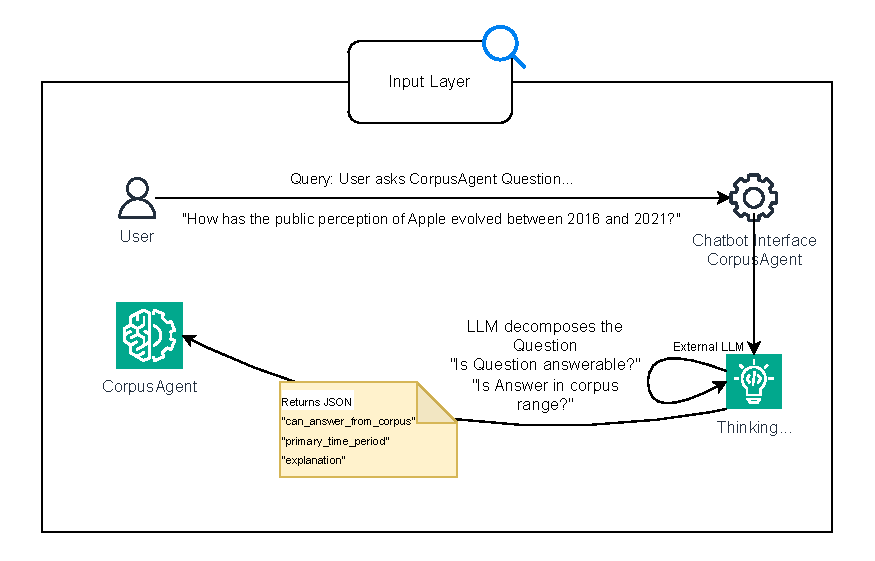
\includegraphics[width=1\textwidth]{Figures/input-layer.pdf}
    \caption{Input Layer (own illustration)}
    \label{fig:input-layer}
\end{figure}

The entry point of the CorpusAgent system is the Input Layer, as illustrated in Figure \ref{fig:input-layer}. It is responsible for receiving user queries, validating them, and performing any necessary preprocessing before passing them on to the subsequent layers.

The interaction begins when a user submits a natural language question through the chatbot interface of our CorpusAgent system. These questions are typically high-level analytical queries that may span over mutliple years and require aggregation or interpretation over a large corpus of documents.

Upon receiving a query, the Input Layer forwards it to an either external or internal Large Language Model (LLM) for an initial reasoning step. At this stage, the LLM does not attempt to generate a final answer. Instead, it performs a lightweight decomposition and feasibility assessment of the query. Specifically, it evaluates whether the question falls within the temporal and thematic scope of the indexed data.

The motivation behind this design decision is to introduce an explicit reasoning and validation step at the very beginning of the pipeline. By performing an initial feasibility assessment, the system can identify questions that cannot be meaningfully answered using the available corpus, for example due to missing temporal coverage or insufficient data. This early filtering prevents unnecessary downstream processing and ensures that subsequent pipeline stages operate only on well-scoped and answerable queries.

The outcome of the assessment is a structured JSON format containing whether the question is answerable, the primary time period of interest and a short explanation justifying the decision.



%-----------------------------------
% Multi-Stage Planning Layer
%-----------------------------------

\subsection{Multi-Stage Planning Layer}
\label{PipelinePlanningLayer}

\begin{figure}[ht]
    \centering
    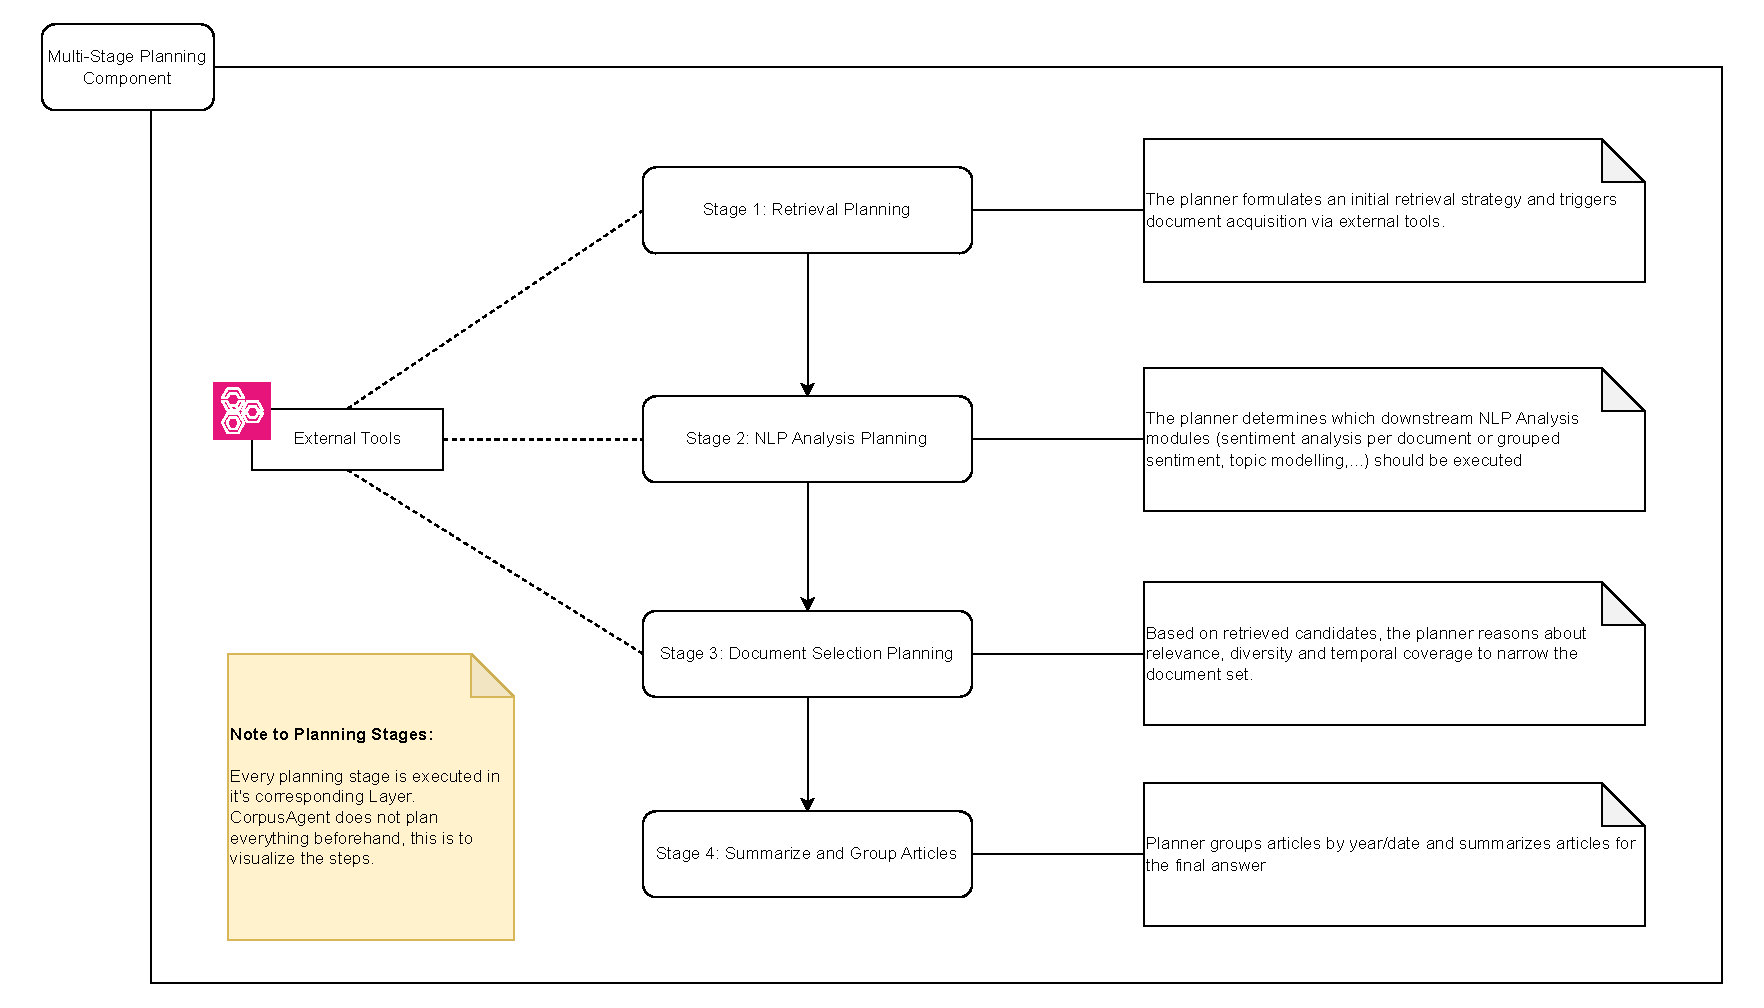
\includegraphics[width=1\textwidth]{Figures/planning-layer.pdf}
    \caption{Planning Layer (own illustration)}
    \label{fig:planning-layer}
\end{figure}

The Multi-Stage Planning Layer is responsible for orchestrating the overall problem-solving strategy of the CorpusAgent systeem. Contrary to the other layers, this layer is rather integrated into each of the other layers instead of being a standalone module as illustrated in Figure \ref{fig:planning-layer}. Rather than following a fixed, hard-coded execution path, this module introduces an agentic control mechanism in which a Large Language Model (LLM) dynamically determines how a given query should be processed across the various pipeline layers.

At this stage, the LLM is provided with a set of available external tools it can execute. These tools consist of function calls such as retrieval, natural language processing (NLP) analyses, document filtering and answer synthesis. However, the specific decisions regarding which tools to invoke, in what order and how many times are delegated to the LLM itself. Rather than a rigid sequence of operations, the planning layer enables a flexible, adaptive approach where the LLM can iteratively refine its strategy based on intermediate results. This design choice allows the system to adapt its strategy to the nature and complexity of the input query and can lead to multiple strategies for the same question.

What makes this approach particularly powerful is that the decision-making authority is not limited to a single planning step. Instead, the LLM is invoked after each major pipeline stage to reassess the current state of the task and determine the next best approach.

Each stage operates as a controlled execution step, while the overall reasing flow is handled by the LLM's conextual understanding ot the task. This agentic, multi-stage planning approach enables our system to handle a wide range of analytic queries with varying results.

The first concrete execution step is determined by the LLM is the retrieval of the relevant documents, which is described in the next section.


\subsection{Retrieval Layer}

\begin{figure}[ht]
    \centering
    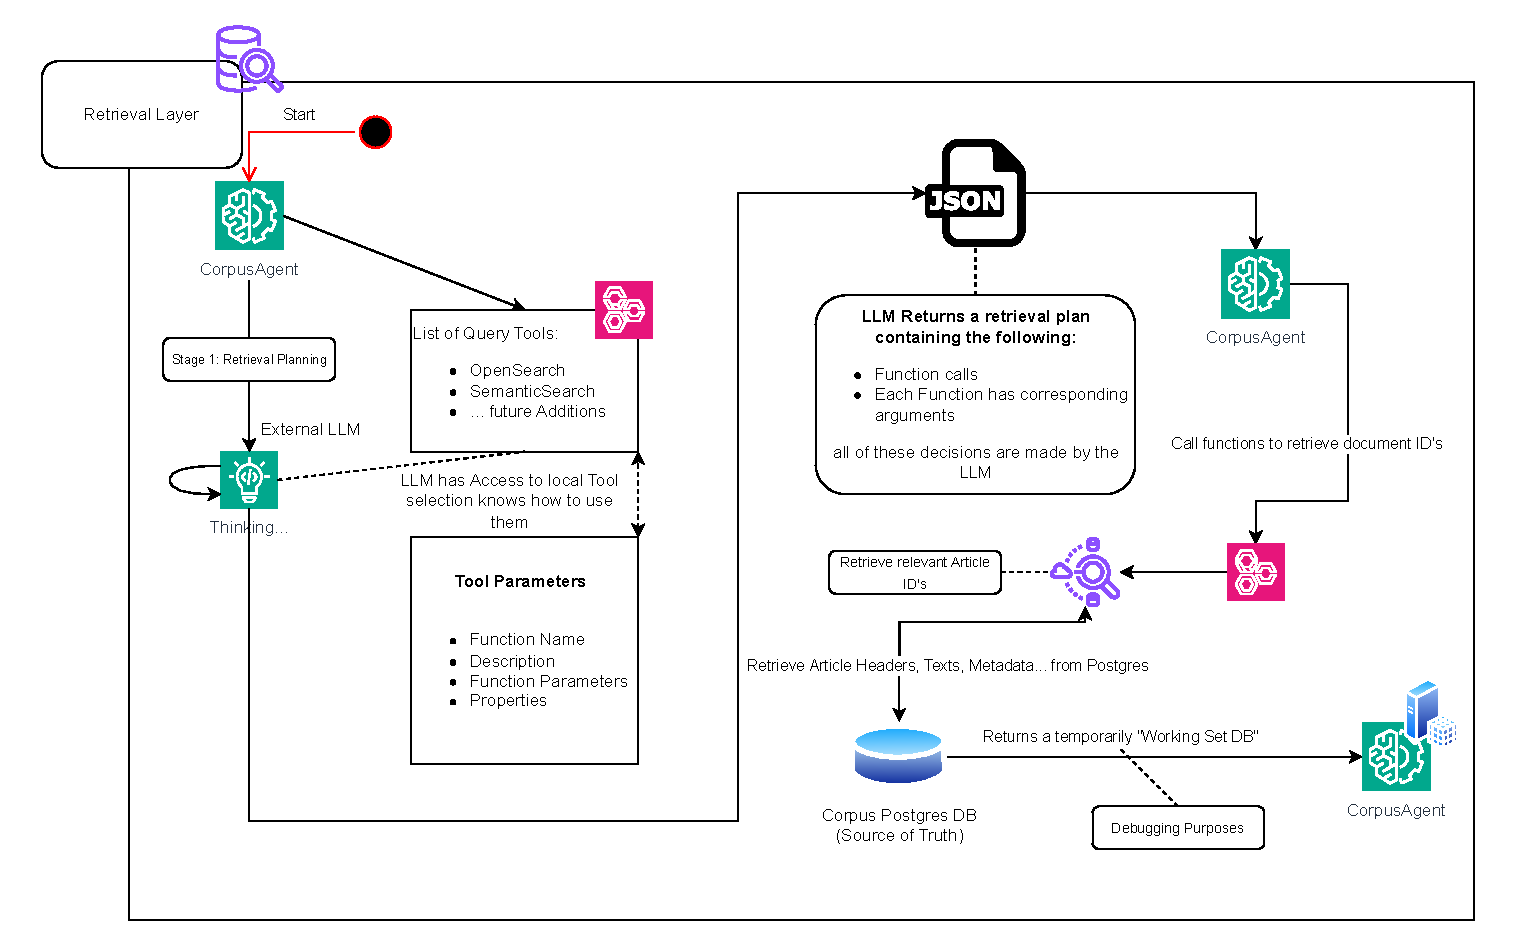
\includegraphics[width=1\textwidth]{Figures/retrieval-layer.pdf}
    \caption{Retrieval Layer (own illustration)}
    \label{fig:retrieval-layer}
\end{figure}

The Retrieval Layer is responsible for identifying and collecting a set of documents that are potentially relevant to the user’s query. Its primary goal is to efficiently reduce the overall corpus to a manageable subset that can be further analyzed by subsequent pipeline stages. An overview of this process is illustrated in Figure \ref{fig:retrieval-layer}.

As like with the other layers, the retrieval process is guided by the retrieval planning decisions made by the Large Language Model. The LLM determines here the appropriate retrieval strategy based on the user query and provided toolset. Rather than directly accessing the data itself, the LLM generates a structured retrieval plan in the form of one or more function calls. These function calls specify which retrieval tools should be used, the corresponding query expressions, and additional parameters such as the number of documents to return. All retrieval related decisions, including whether multiple retrieval calls are required, for example to cover different time periods, are made by the LLM.

Currently, the primary retrieval backend is OpenSearch, which is used to index the news corpus and enable fast full-text search. OpenSearch is based on the Lucene engine and relies on inverted indices, allowing keyword-based queries to be executed significantly faster than traditional relational database text matching. In preliminary experiments, this approach was empirically validated by comparing OpenSearch queries against SQL-based text search using \texttt{LIKE} expressions in PostgreSQL, where OpenSearch consistently produced substantially faster query execution times for large text collections. Which is to be expected given the underlying indexing mechanisms.

The use of OpenSearch at this stage is not only motivated by performance considerations but also by extensibility. The retrieval interface is designed in such a manner, such that additional retrieval mechanisms such as semantic vector search or alternative indexing systems can be integrated in the future without requiring fundamental changes to the architecture.

An example of a retrieval function call generated by the LLM is shown below:

\begin{lstlisting}[language=json, caption={Example OpenSearch retrieval function call}, label={lst:opensearch-call}]
{
  "id": "call_VBCxxwHwvAluJHuoMOrdC6iF",
  "type": "function",
  "function": {
    "name": "search_opensearch",
    "arguments": {
      "query": "Bitcoin (\"public perception\" OR \"public opinion\" OR sentiment OR adoption OR \"mainstream\" OR bubble OR scam OR regulation OR investment) 2016",
      "top_k": 50
    }
  }
}
\end{lstlisting}

Such function calls like the one shown in Listing \ref{lst:opensearch-call} are generated by the LLM based on the entire context provided to it, including the user query. These are then returned to the CorpusAgent in a structured JSON format. The CorpusAgent executes all the specified function calls and collects the resulting documents.

The system eomploys both a PostgreSQL database and an OpenSearch index to balance data integrity, flexibility and retrieval performance. Here we use PostgreSQL as the primary data store and authoritative source of truth for all news articles and associated metadata. The reason behind this design choice is to ensure that the complete and consistent dataset is maintained in a robust relational database system.

Using a relational database as the main data source also provides more flexibility for future extensions of the news corpus or completely new datasets. Different datasets may have additional metadata beyond the basic fields such as headlines and article text. Such attributes may be relevant for downstream analysis or filtering steps but not necessarily suitable or required for indexing in OpenSearch. Maintaining these attributes in PostgreSQL allows the system to evolve without requiring changes to the indexing structure.

Therefore OpenSearch is used as a secondary, specialized component optimized for large scale text retrieval. Separating these concerns allows the system to combine the strengths of both technologies, having a reliable primary data store while leveraging the performance benefits of a dedicated search engine for text retrieval tasks.

In addition to these persisent data stores, the system maintains a temporary, per-run working database that archives all retrieved documents and intermediate NLP outputs generated during a single pipeline execution. The purpose of this temporary dataset is primarily intended for debugging, analysis and result validation. Given the exploratory and analytical nature of the task, determining whether a generated answer is correct is inherently challenging. Instead of relying solely on the final answers, this design allows the the user to inspect the entire processing history, including which documents were retrieved and how they were analyzed. This transparency facilitates error analysis and helps identify potential issues in the retrieval or processing steps. Not to mention, it allows the user to assess whether the final answer is grounded in the retrieved evidence rahter than relying on unsupported or hallucinated information.

% TODO : Add a SQL Database Schema Figure
\subsection{Analytics Layer}

\begin{figure}[ht]
    \centering
    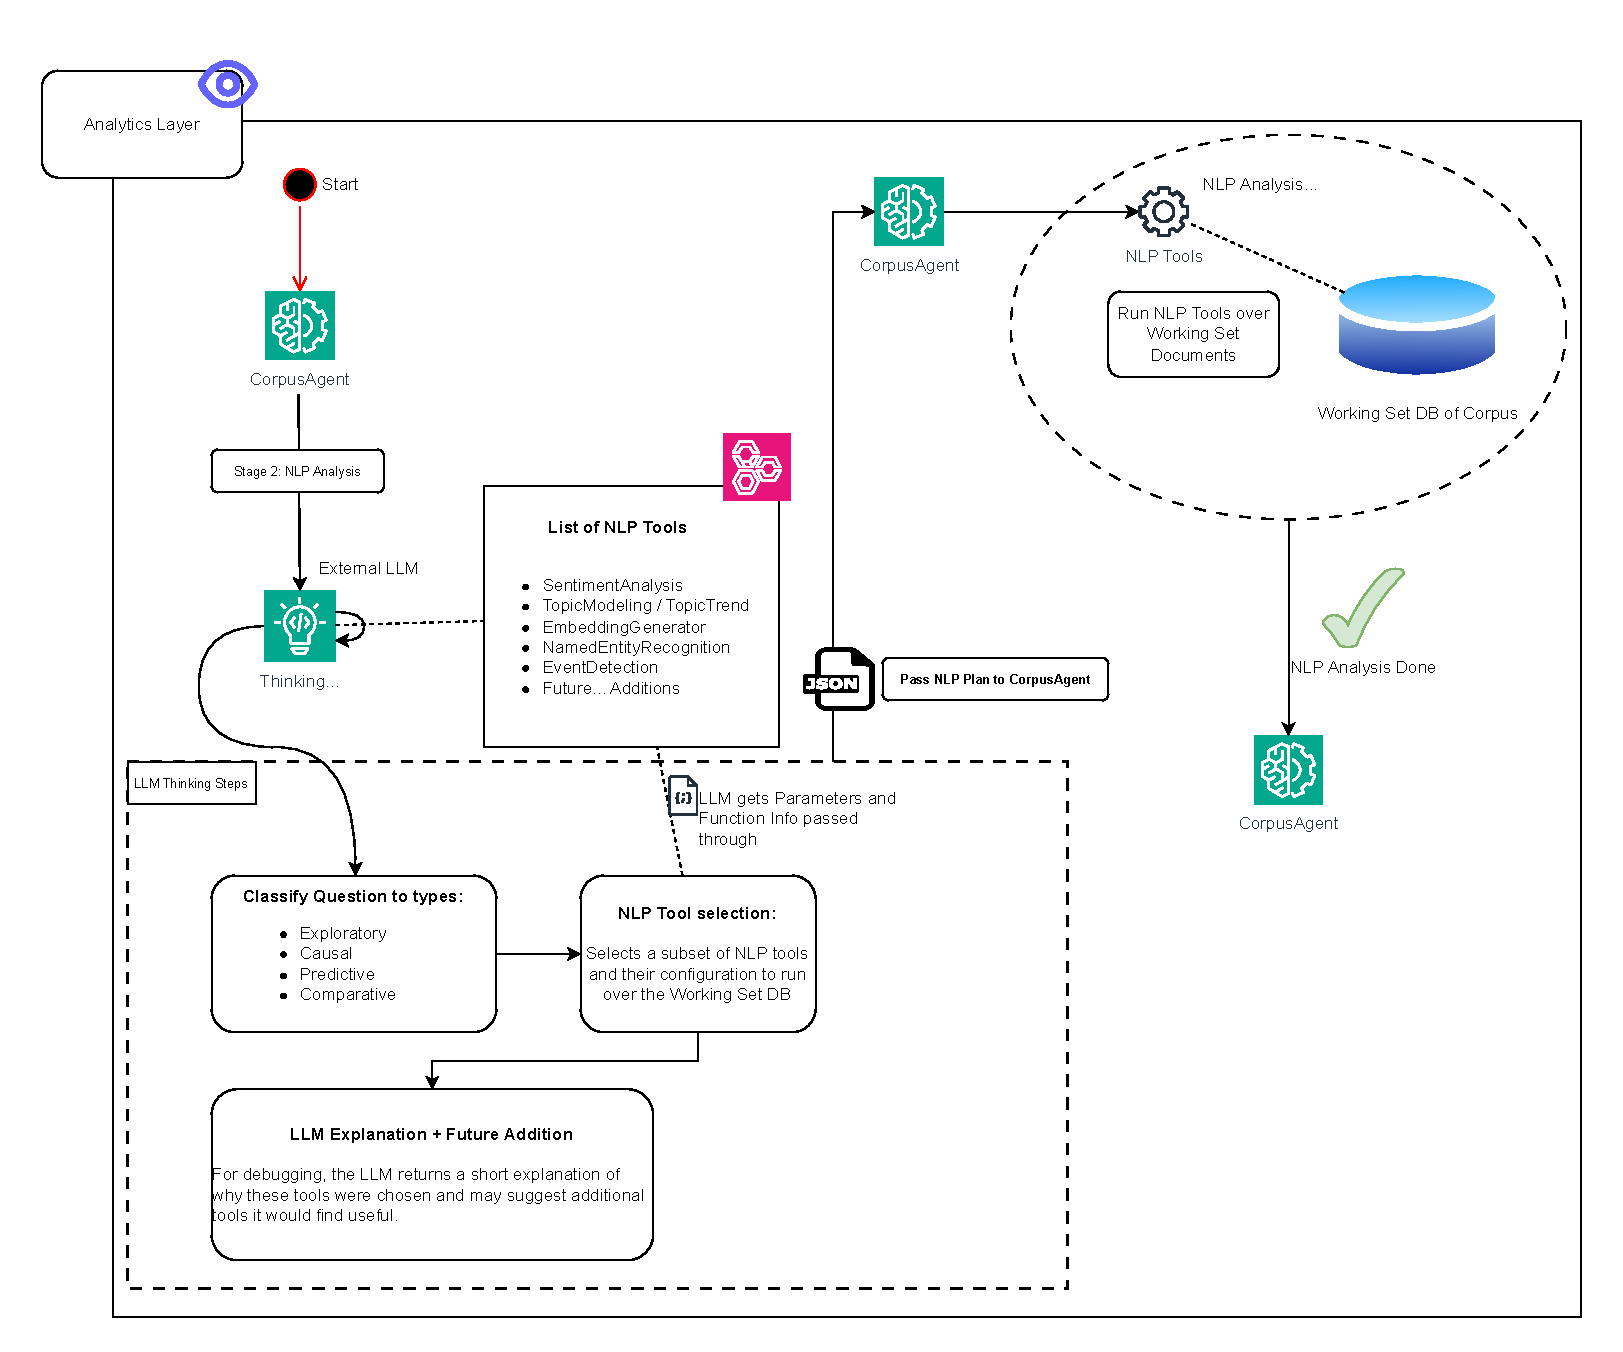
\includegraphics[width=1\textwidth]{Figures/analytics-layer.pdf}
    \caption{Analytics Layer (own illustration)}
    \label{fig:analytics-layer}
\end{figure}

The Analytics Layer is responsible for applying targeted natural language processing (NLP) methods to the working set of documents retrieved in the previous stage. Primarily, its objective is to extract structured signals from unstructured text that support higher-level analytical reasoning, such as identifying trends, sentiments, entities, or events over time. An overview of this process is illustrated in Figure~\ref{fig:analytics-layer}.

At the beginning of this layer, the Large Language Model (LLM), guided by the Multi-Stage Planning Layer, determines which analytical tools are appropriate for the given query. Rather than executing all available NLP methods indiscriminately, the system adopts a selective approach in which the LLM first classifies the nature of the question, for example as exploratory, comparative, predictive, or causal. Based on this classification, the LLM selects a subset of NLP tools and configures their parameters accordingly. Additionally, we prompt the LLM to provide a brief explanation of why specific tools were chosen, which serves as documentation for the analytical strategy. Furthermore we ask the LLM to suggest any additional tools that could be relevant for future iterations, even if they are not executed in the current run.


The applied NLP methods represent well-established techniques for extracting structured information from large text corpora, including sentiment analysis, topic modeling, named entity recognition, and event detection. Such techniques have been extensively studied and applied in prior work on text analytics and information extraction \cite{jurafsky2023slp, blei2003lda, pang2008sentiment}.

Currently in this concept phase, we have only mocked the actual implementation of these NLP tools. However, in a fully realized system, each selected tool would be executed over the temporary working dataset produced by the Retrieval Layer. The outputs of these analyses would then be stored back into the working database, enriching the document set with structured annotations that can be leveraged in subsequent processing steps.

Depending on the type of analysis, the NLP Outputs are either stored per article (e.g., sentiment scores, named entities) or when there are cross-document results (e.g., topics, event clusters), they are stored in separate tables linked to the relevant articles. This structured storage approach allows for efficient querying and aggregation of analytical results during later stages of the pipeline.


All selected NLP tools are executed over the temporary working dataset produced by the Retrieval Layer. By operating on this reduced document set, the system avoids unnecessary computation over the full corpus while still retaining sufficient contextual coverage for meaningful analysis. The LLM specifies tool selections, execution order, and configuration parameters in a structured JSON format, which is subsequently interpreted and executed by the CorpusAgent.

Once all selected NLP analyses have been completed, the enriched working dataset is passed to the Document Selection and Filtering Layer for further refinement.

\pagebreak

\subsection{Document Selection / Filtering Layer}

\begin{figure}[ht]
    \centering
    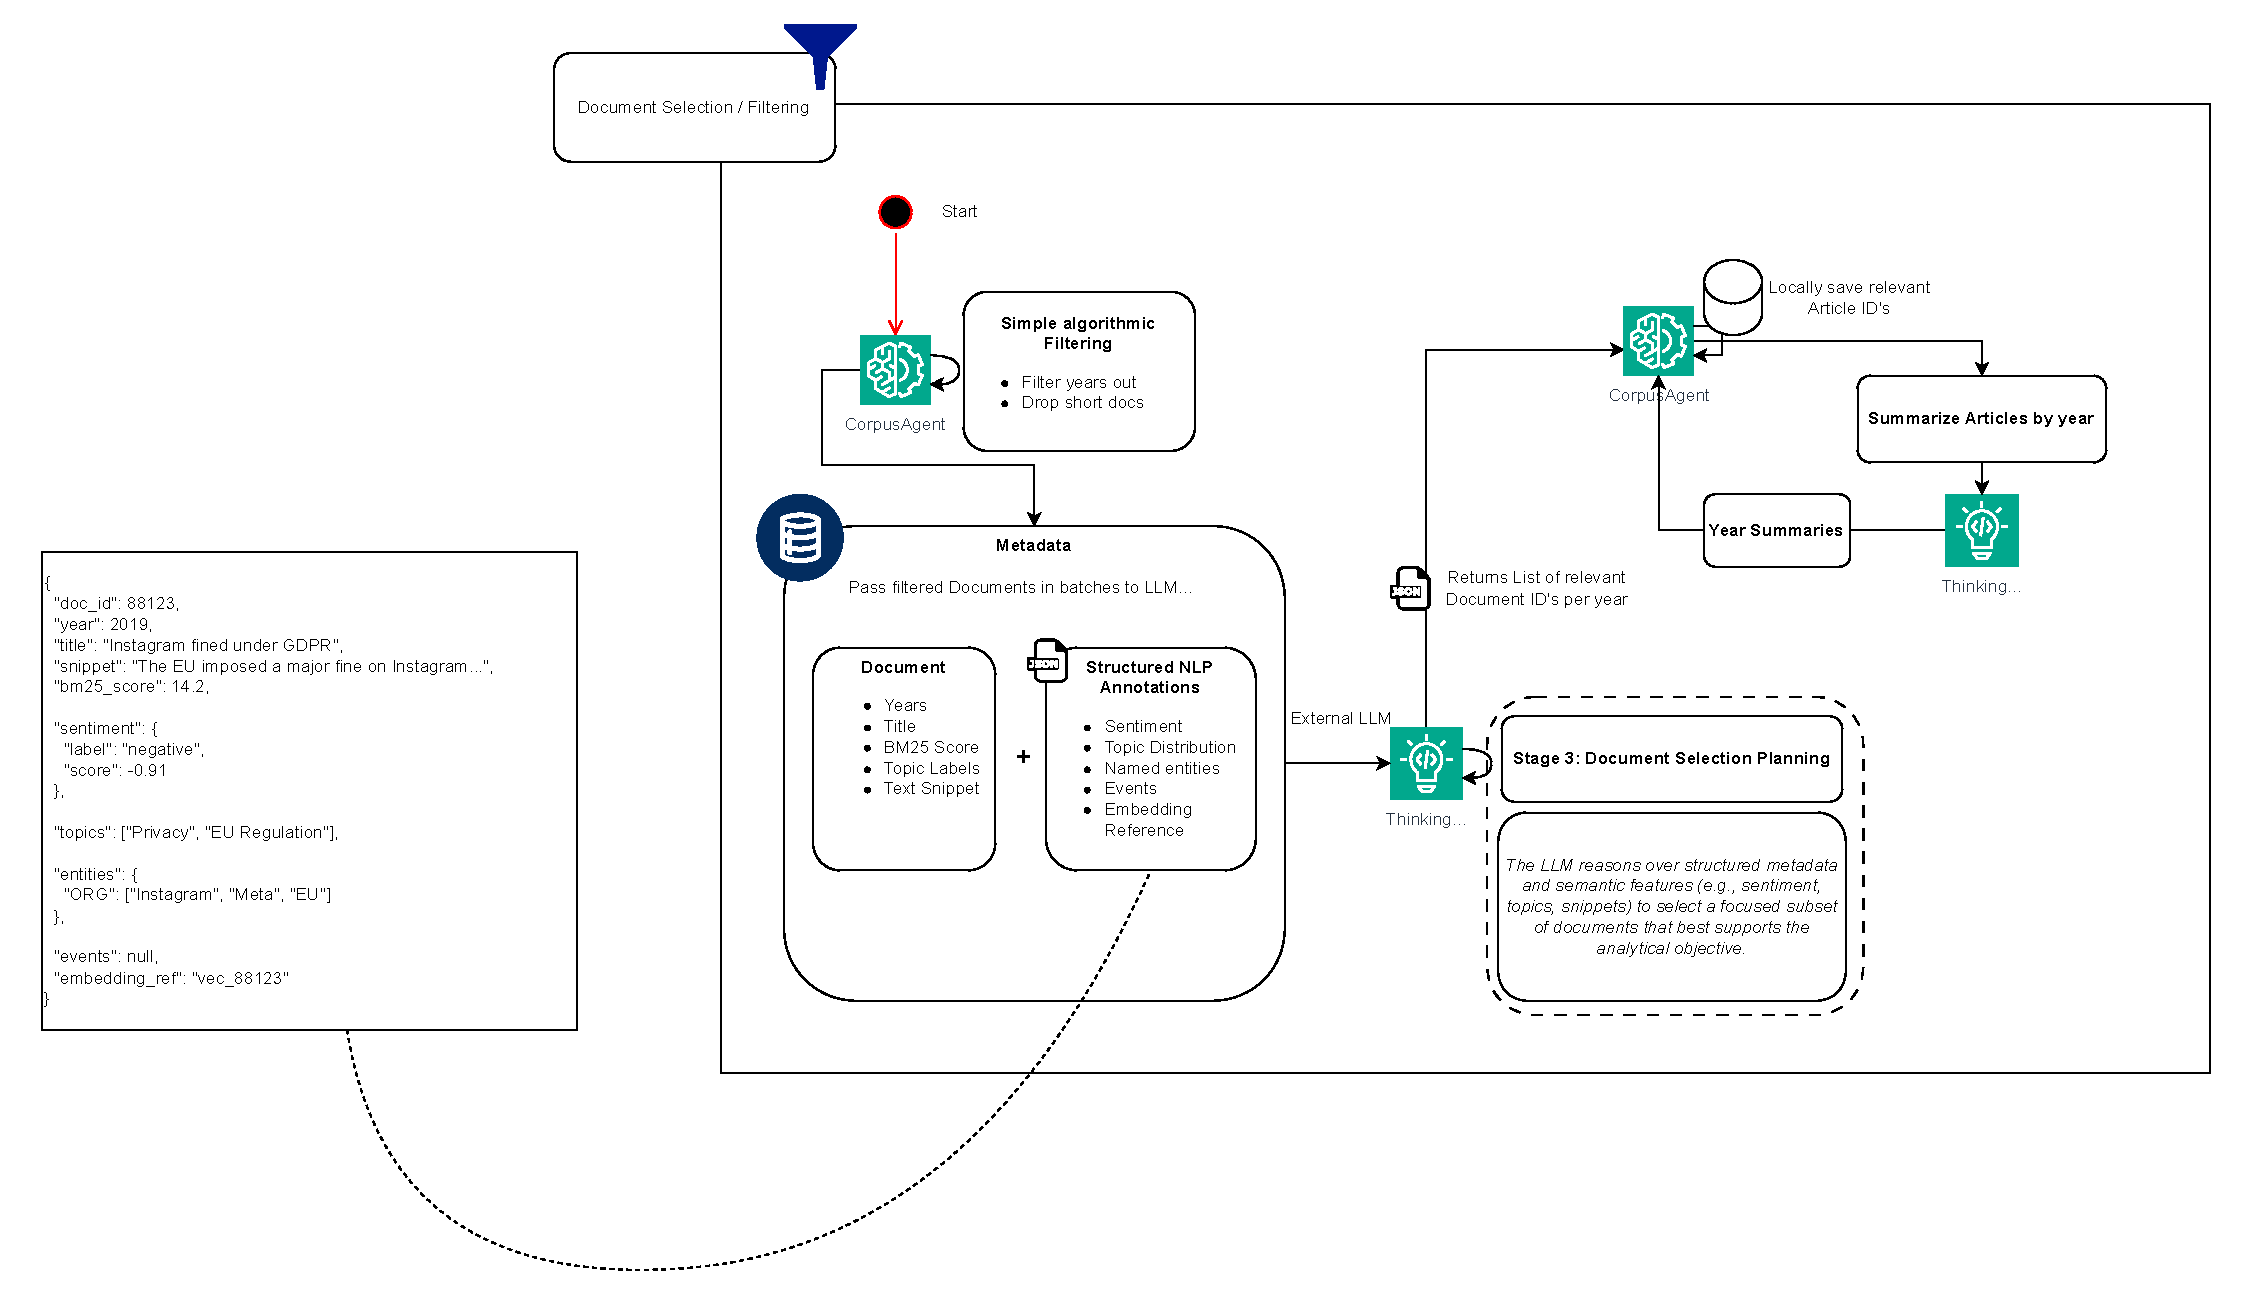
\includegraphics[width=1\textwidth]{Figures/document-filtering.pdf}
    \caption{Document Selection / Filtering Layer (own illustration)}
    \label{fig:document-filtering-layer}
\end{figure}

The Document Selection and Filtering Layer is responsible for refining the analytically enriched working dataset to a focused subset of documents that most effectively support the final answer synthesis. Previous pipeline stages were primarily concerned with broad retrieval and comprehensive analysis. In contrast, this layer aims to distill the dataset down to the most relevant and informative documents. An overview of this process is illustrated in Figure \ref{fig:document-filtering-layer}.

Here the filtering process first off begins with a lightweight, deterministic pre-filtering step directly inside the CorpusAgent. This step applies simple algorithmic criteria to eliminate documents that are clearly irrelevant or low-quality. Such criteria may include removing duplicates, filtering out articles below a certain length, or excluding documents that do not meet the time horizon of the task. This initial pruning helps reduce noise and focuses subsequent processing on a more manageable set of candidates.

After this initial pre-filtering, the refined working dataset is represented in a structured format that combines retrieved metadata and analytical annotations from the analytical layer. This structured representation includes among other attributes, the publication year, title, full article text, retrieval score (e.g. BM25), sentiment score and label and identified named entities. These attributes can vary depending on the specific NLP tools applied in the previous layer.

In this next step, the CorpusAgent forwards these document representations in batches to the Large Language Model (LLM). Instead of selecting documents based on fixed attributes like retrieval scores or sentiment thresholds, we prompt the LLM to reason with the initial user query in mind, to determine which documents are most important to answering the question.

As a result, the LLM evalutes in each batch which documents are most relevant and informative for the specific analytical task. The selected document IDs are then returned to the CorpusAgent in a structured JSON format with once again an explanation of why these documents were chosen. Inside the temporary working database, the CorpusAgent marks these documents as selected for inclusion in the final answer synthesis.

Finally, once all documents have been processed, the CorpusAgent once again prompts the LLM to generate a summary of each year represented in the selected documents. These yearly summaries provide a concise overview of the key themes, events, and trends identified in the filtered dataset. They also serve to reduce the overall context length required for the final answer synthesis step, as only the summaries rather than the full articles need to be considered.

Our motivation behind this layer was to introduce a human-like judgment step into the pipeline. Rather than relying solely on algorithmic criteria, we leverage the LLM's contextual understanding to make nuanced decisions about document relevance. This approach allows the system to adaptively focus on the most pertinent information for each unique query, ultimately improving the quality and accuracy of the final synthesized answers.

With the selected documents and yearly summaries prepared, the pipeline is now ready to proceed to the final stage: LLM Answer Synthesis.

\subsection{LLM Answer Synthesis}

\begin{figure}[ht]
    \centering
    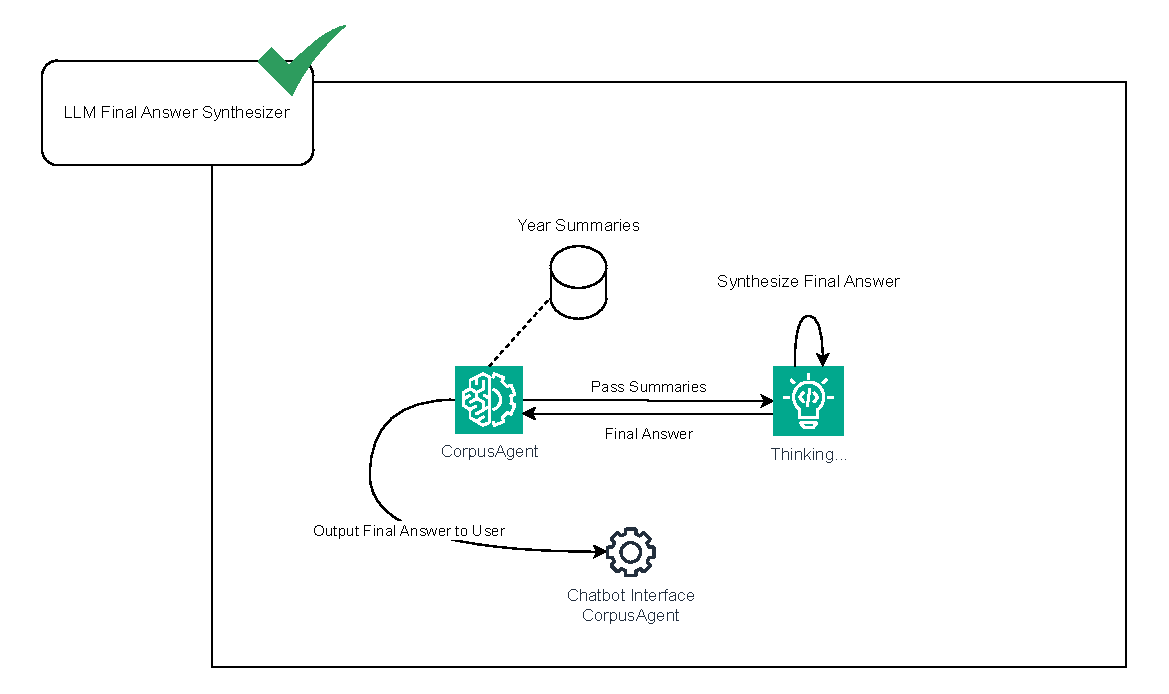
\includegraphics[width=1\textwidth]{Figures/final-synthesize.pdf}
    \caption{LLM Answer Synthesis Layer (own illustration)}
    \label{fig:llm-answer-synthesis-layer}
\end{figure}

The final stage of the CorpusAgent pipeline is the LLM Answer Synthesis Layer, as illustrated in Figure \ref{fig:llm-answer-synthesis-layer}. This layer is responsible for generating a coherent, well-structured answer to the user's original query based on the refined set of documents and analytical insights produced by the preceding layers. Combined with the input layer, these two layers are the only parts of the pipeline that directly interact with the user. At this point, the system relies solely on the condensed, temporally organized summaries that capture the most relevant information extracted from the corpus.

The CorpusAgent passes the yearly summaries derived from the Documen Selection phase before to the LLM along with the original user query. Additionally, we provide even further context if available, such as NLP outputs that may span over multiple documents (e.g., identified trends or events). The LLM is then prompted to synthesize this information into a comprehensive answer that directly addresses the user's question.

The synthesis process focuses on identifying overarching patterns, temporal developments, and meaningful comparisons across time periods. For example, shifts in sentiment, changes in dominant topics, or the emergence of new narratives can be explicitly highlighted and related back to the original analytical question. The resulting output is a single, consolidated answer that integrates insights across all relevant years.

Finally, the synthesized answer is returned to the user through the chatbot interface of the CorpusAgent system. By separating answer generation from retrieval, analysis, and document selection, this layer provides a clear abstraction boundary and ensures that the final response can be traced back to specific intermediate representations. This transparency is crucial for validating the correctness and reliability of the generated answers, especially in complex analytical scenarios.

\pagebreak

%-----------------------------------
% Visualization Playground
%-----------------------------------

\section{Visualization Playground (Auxiliary Component)}

\begin{figure}[ht]
    \centering
    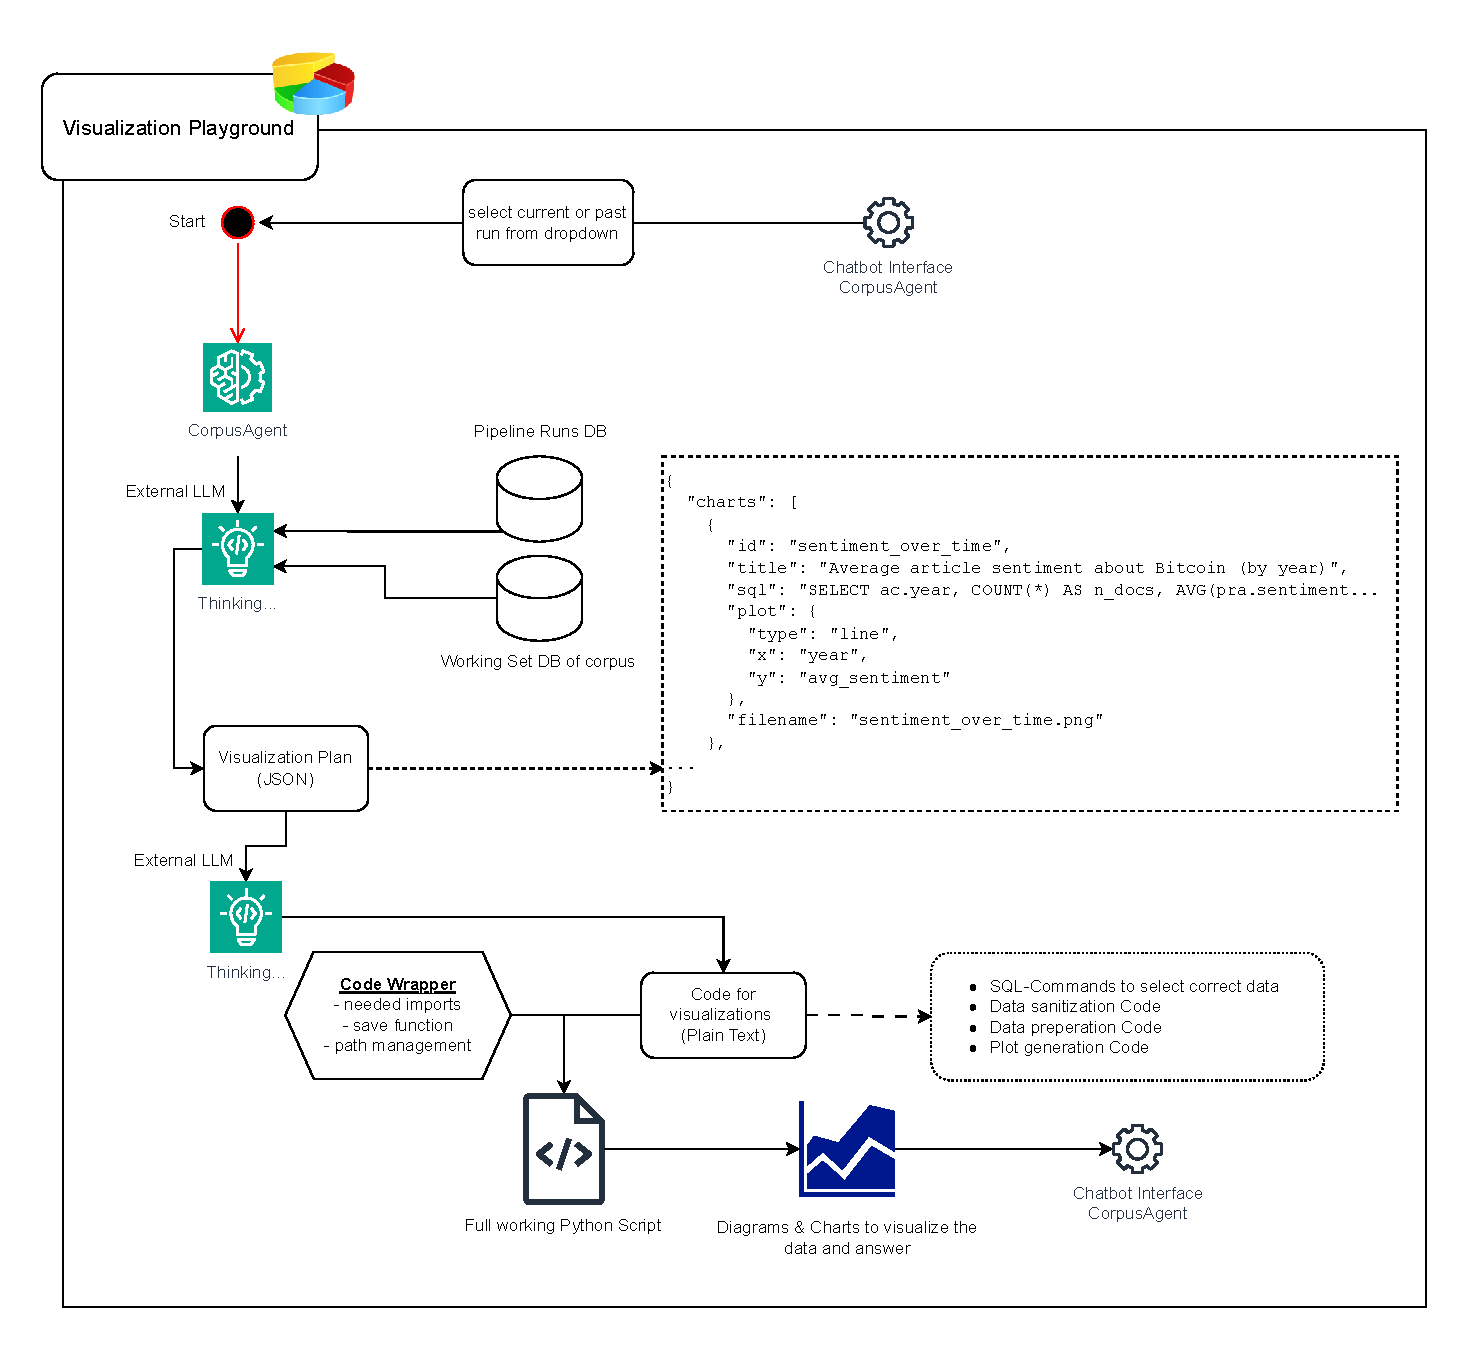
\includegraphics[width=1\textwidth]{Figures/visualization-playground.pdf}
    \caption{Visualization Playground (own illustration)}
    \label{fig:visualization-playground}
\end{figure}

The CorpusAgent pipeline is designed to answer complex analytical questions over large news corpora by decomposing the task into retrieval, analysis, filtering, and synthesis stages. \\
However, corpus-level analytics are difficult to validate purely from a final textual answer. Users typically need to inspect temporal trends, distributions, and supporting evidence to judge whether the answer is grounded in the retrieved material. Also, visualizations can help communicate complex patterns more effectively than text alone.
To support this requirement, we implemented a Visualization Playground as an auxiliary component that generates plots and diagrams on demand for a selected pipeline run.
Conceptually, the playground consumes two persistent information sources:

\begin{itemize}
    \item The authoritative corpus and per-run working set stored in PostgreSQL
    \item The pipeline run metadata and outputs (e.g., question, final answer, and structured intermediate artifacts) stored in a separate run database
\end{itemize}

Based on this input, the system produces a visualization plan (structured JSON), generates executable plotting code, and renders the resulting images as reproducible artifacts that can be inspected inside the interface.

This design mirrors the high-level workflow shown in the Figure \ref{fig:visualization-playground}: an LLM produces a JSON visualization specification and plotting code which is executed to create charts saved as run artifacts.

\subsection{Data Sources and Run Selection}

The playground is run-centric: the user selects a run\_id corresponding to a previously executed pipeline run. \\
The implementation provides a small run management module that lists recent runs and fetches detailed run information from the pipeline\_runs table, including fields such as question, final\_answer, and additional stored debug artifacts. These run-level fields serve two purposes:

\begin{enumerate}
    \item Semantic context for the visualization planner and code generator (the LLM is conditioned on what the run was trying to answer).
    \item Traceability since produced charts can always be linked back to an immutable run identifier.
\end{enumerate}

In addition to run metadata, the playground queries the per-run working dataset stored in pipeline\_run\_articles (linked to the main corpus table article\_corpus). The design intentionally queries only a reduced, run-specific slice rather than the entire corpus to keep visualization computation bounded and directly relevant to the specific question.

\begin{lstlisting}[caption={Example DB schema summary}, label={lst:db-schema}]
article_corpus(id bigint, year smallint, source_domain text, title text, body text)

pipeline_run_articles(run_id uuid, question text, article_id bigint, rank integer, os_score real, sentiment_score real, relevance_score real, extra_metadata jsonb)

pipeline_runs(run_id uuid, question text, nlp_plan jsonb, mocked_tool_outputs jsonb, final_answer text, created_at timestamp with time zone)
\end{lstlisting}

\subsection{LLM-Based Visualization Planning}

The first step is planning: given (question, final\_answer, run\_id), the planner asks the LLM to propose a set of charts expressed as a JSON structure. \\
Each chart entry contains: a stable identifier \textit{id}, a human-readable \textit{title}, an SQL query string \textit{sql}, a minimal plot specification \textit{plot} (e.g. type, x, y) and an output \textit{filename} (PNG).

This plan is explicitly constrained to valid JSON via structured response formatting (JSON object), which makes downstream handling deterministic (e.g., rendering the plan in the UI, validating presence of required fields). The planner prompt also injects a compact schema summary so the model does not need to guess table/column names.

The full JSON plan can be inspected before proceeding to code generation, allowing the user to verify that the proposed charts align with their expectations.

\begin{lstlisting}[caption={Example Visualization Plan JSON}, label={lst:viz-plan}]
{
    "charts": [
        index : {
            "id": "...",
            "title": "...",
            "sql": "... WHERE pra.run_id = :run_id ...",
            "plot": { "type": "line|bar", "x": "...", "y": "..." },
            "filename": "...png"
        },
        ...
    ]
}
\end{lstlisting}

A key design concern is the presence of \textit{extra\_metadata} stored as JSONB, which varies between runs. To reduce hallucinated JSON keys, the planner additionally includes a glimpse of observed JSON key paths and examples extracted from the selected run. The LLM is instructed to use only those keys and to query JSONB via Postgres JSON operators when needed.

\subsection{LLM-Based Code Generation}

The visualization plan is intentionally lightweight. It is primarily meant for transparency and for guiding the next step: code generation. \\
In the second step, the system prompts the LLM to generate Python plotting code that queries the PostgreSQL database and produces PNG charts using Matplotlib. The code generator is constrained through explicit rules, including:

\begin{itemize}
    \item return only Python code (no markdown)
    \item use Matplotlib (avoid additional plotting dependencies)
    \item obtain data via a provided \textit{query\_df(sql, params)} helper
    \item save output figures only through a provided \textit{save\_fig(fig, filename)} function
\end{itemize}

This separation (plan → code) is deliberate: the plan acts as a structured, inspectable intermediate representation, while the code step is responsible for the full procedural details (data preparation, grouping/aggregation, plotting, labeling, and exporting).
It also helps preventing hallucinated Code regarding paths, run\_id usage, and saving conventions.

\subsection{Controlled Execution and Artifact Management}

To execute LLM-generated code while keeping the system reproducible and debuggable, the playground runs the generated script via a wrapper-based execution mechanism:
\begin{enumerate}
    \item The user-generated code is written to an artifact directory under the selected run\_id.
    \item A wrapper script is created which injects:
          \begin{itemize}
              \item environment-backed values (RUN\_ID, OUT\_DIR)
              \item the database query helper query\_df
              \item and a constrained \textit{save\_fig} routine that validates .png filenames and writes output into OUT\_DIR
          \end{itemize}
    \item The wrapper is executed in a subprocess with an explicit timeout to prevent runaway code.
    \item Standard output/error are captured into log files.
    \item All produced PNGs are collected from the artifact directory and displayed in the interface.
\end{enumerate}

Artifacts are stored in a structured directory layout (e.g., artifacts/visuals/<run\_id>/...) to ensure that every generated visualization is reproducible and attributable to a run. \\
Since this feature is heavily volatile, due to LLM code generation, persisting the generated code and execution logs is also crucial for failure analysis: when plots fail to render (e.g., SQL errors, schema mismatches, missing fields), the developer can directly inspect the exact script, stdout, and stderr of the run.

\begin{lstlisting}[language=Python, caption={Safety and reproducibility wrapper for executing LLM-generated plotting code}, label={lst:code-exec-wrapper}]
import os
from pathlib import Path
import matplotlib.pyplot as plt

from viz.db import query_df  # SQLAlchemy-based query_df

# path setup
RUN_ID = os.environ.get("RUN_ID")
OUT_DIR = Path(os.environ.get("OUT_DIR", ".")).resolve()
OUT_DIR.mkdir(parents=True, exist_ok=True)

# constrained save_fig implementation
def save_fig(fig, filename: str) -> str:
    if not filename.endswith(".png"):
        raise ValueError("filename must end with .png")
    path = (OUT_DIR / filename).resolve()
    fig.savefig(path, dpi=160, bbox_inches="tight")
    plt.close(fig)
    return str(path)

# --- user code below ---
run_id = RUN_ID
{user_code}
\end{lstlisting}

